% Created 2020-09-07 Mon 23:17
% Intended LaTeX compiler: lualatex
\documentclass[11pt]{article}
\usepackage{graphicx}
\usepackage{grffile}
\usepackage{longtable}
\usepackage{wrapfig}
\usepackage{rotating}
\usepackage[normalem]{ulem}
\usepackage{amsmath}
\usepackage{textcomp}
\usepackage{amssymb}
\usepackage{capt-of}
\usepackage{hyperref}
\usepackage{tabularx}
\usepackage{etoolbox}
\makeatletter
\def\dontdofcolorbox{\renewcommand\fcolorbox[4][]{##4}}
\AtBeginEnvironment{minted}{\dontdofcolorbox}
\makeatother
\usepackage[newfloat]{minted}
\usepackage{pdfpages}
\author{Mark Armstrong}
\date{August 2nd, 2020}
\title{Computer Science 3MI3 - Principles of Programming Languages\\\medskip
\large 2020 Course Outline}
\hypersetup{
   pdfauthor={Mark Armstrong},
   pdftitle={Computer Science 3MI3 - Principles of Programming Languages},
   pdfkeywords={},
   pdfsubject={The course outline for the 2020 class of 3mi3.},
   pdfcreator={Emacs 27.0.90 (Org mode 9.3.7)},
   pdflang={English},
   colorlinks,
   linkcolor=blue,
   citecolor=blue,
   urlcolor=blue
   }
\begin{document}

\maketitle
\tableofcontents


\section{TL;DR (Too Long, Didn't Read)}
\label{sec:org340fdf8}
At the very least, please review these sections of the outline.
\begin{itemize}
\item \hyperref[sec:orgafe5439]{Course staff}
\item \hyperref[sec:org2eb9cb9]{Communicating with course staff}
\item \hyperref[sec:orgc848c7d]{Your responsibilities regarding course administration tools}
\item \hyperref[sec:org83d497e]{Asking well-posed questions}
\item \hyperref[sec:org015c739]{Grading},
\begin{itemize}
\item \hyperref[sec:orgd83cfff]{Missed work},
\item \hyperref[sec:org116bd17]{Homework due dates} and
\item \hyperref[sec:orge86e1b9]{Assignment due dates}.
\end{itemize}
\end{itemize}

\section{The purpose of an outline}
\label{sec:orgf2f7810}
\begin{quote}
“A course outline sets the expectations for students
and what they can expect in terms of the course
experience they will receive,
the format in which the course will be delivered
and the knowledge and skills that can be gained.
The outline introduces the course and the instructor
and sets out the expectations of the instructor
so that students are aware of how they will learn,
what level of participation will be expected
and how they will be assessed.”
\end{quote}

\section{Course staff}
\label{sec:orgafe5439}
\subsection{Instructor: Mark Armstrong}
\label{sec:orgfcef033}
\begin{quote}
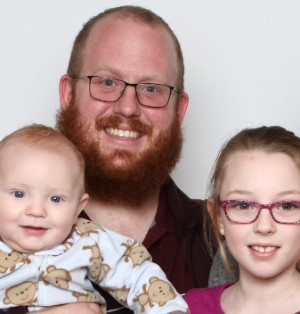
\includegraphics[width=200px]{./media/markarmstrong.jpg}
\end{quote}

\begin{itemize}
\item Email: \url{mailto:armstmp@mcmaster.ca}
\item Website: \url{https://armkeh.github.io}
\end{itemize}
\subsection{Teaching assistants}
\label{sec:org5149316}
:TODO:

\section{Schedule}
\label{sec:org4aa836a}
\begin{center}
\begin{tabular}{|l|l|l|l|l|l|l|l|}
\hline
 & Mon & Tues & Wed & Thu & Fri & Sat & Sun \\
\hline
9:30 & & & Tutorial 2 & & & & \\
\hline
10:30 & & & & & & & \\
\hline
11:30 & Lecture & & Lecture & & & & \\
\hline
12:30 & Tutorial 1 & & & & & & \\
\hline
13:30 & & & & & Lecture & & \\
\hline
EOD & & & & & Homework & & Homework \\
 & & & & & released & & due \\
\hline
\end{tabular}
\end{center}

\subsection{Lecture recordings}
\label{sec:orgb6197b4}
Lectures and tutorials will be made available as recordings
shortly after said lectures and tutorials.

The platform for said recordings will be announced
after the start of classes.
:TODO:

\subsection{Homework due dates}
\label{sec:org116bd17}
This course will have weekly homeworks, as described in \hyperref[sec:org015c739]{Grading}.

Homework will be released each Friday by end of day
and will be due the Sunday nine days later by end of day,
unless a delay is announced on the course homepage,
and except for the weekends surrounding the midterm recess
—there will be a single homework due
the Monday following the recess instead.

\subsection{Assignment due dates}
\label{sec:orge86e1b9}
This course will have three assignments, as described in \hyperref[sec:org015c739]{Grading}.

As of the beginning of the course,
the assignments are planned to be due on
\begin{itemize}
\item October 7th,
\item November 11th, and
\item December 16th.
\end{itemize}

Any changes to these dates will be announced on the course homepage.
Also see \hyperref[sec:orgaf5f3d6]{Accomodations for SAS and conflicts with other courses};
in particular, we will reevaluate the final assignment due date
once the exams schedule is released, based on the exam dates
of other third year computer science courses.

\section{Administration tools}
\label{sec:org6e3ad4a}
\subsection{The tools}
\label{sec:org9b705fb}
This course will be administered via a combination of
\begin{itemize}
\item a “team” on the CAS departmental Microsoft Teams,
\begin{itemize}
\item —Zoom meetings may be used if there is a problem with Teams;
any such change will be announced on the homepage—
\end{itemize}
\item the course
\href{https://armkeh.github.io/principles-of-programming-languages/}{homepage},
\item a \href{https://github.com/armkeh/principles-of-programming-languages}{Github repository}
of the course content, from which
the homepage is hosted as a \texttt{github.io} website,
\item a repository for each student on the
\href{https://gitlab.cas.mcmaster.ca}{McMaster CAS GitLab server}, and
\item communications via McMaster email addresses.
\end{itemize}

Specifically,
\begin{description}
\item[{Teams}] will be used for live lectures\emph{tutorials,
lecture}tutorial recordings,
and preferred for discussions relevant to the whole
(or at least many members of) the class,
\begin{description}
\item[{\textbf{Zoom}}] may be used for live lectures/tutorials
if there are problems with Teams,
\end{description}
\item[{the homepage}] will be used for announcements
and convenient access to notes and homework/assignments,
\item[{the Github repository}] will be used to host the course homepage
and content, and allow students to easily see version changes
to content,
\item[{the Gitlab repository for each student}] will be used
for homework and assignment submissions and grade distribution, and
\item[{McMaster email addresses}] will be used
for private communications with students.
\end{description}

An Avenue to Learn course has been created for this course
for the sake of directing students to the course homepage
and entering homework/assignment deadlines in a calendar.
No course content will be uploaded to Avenue to Learn,
and attempts to communicate with staff on that platform
may go unnoticed and unanswered.

\subsection{Your responsibilities regarding course administration tools}
\label{sec:orgc848c7d}
\textbf{It is the student's responsibility}
\begin{itemize}
\item to ensure they have an account on
the \href{https://gitlab.cas.mcmaster.ca}{McMaster CAS GitLab server} and
the \href{https://teams.microsoft.com/l/team/19\%3a1f2f25fdc5e243d285e2f92216e5b483\%40thread.tacv2/conversations?groupId=a2e98537-757f-4791-b72f-2cf4d7459f28\&tenantId=44376307-b429-42ad-8c25-28cd496f4772}{CAS Microsoft Teams team}
\item to be aware of the information on the course's \href{https://armkeh.github.io/principles-of-programming-languages/}{homepage} and
\item to check the \href{https://armkeh.github.io/principles-of-programming-languages/}{homepage}, their course GitLab repository,
the Microsoft Teams team for the course
and their email regularly for announcements and changes.
\end{itemize}
It is not assumed that students follow the Github repo,
but it is a good practice to stay informed of any and all
changes to content.

\section{Communicating with course staff}
\label{sec:org2eb9cb9}
To communicate with course staff reliably, you should
choose the most appropriate means from the below.
\begin{itemize}
\item “Mention” the course staff member in a relevant channel on
the Microsoft Teams team.
\begin{itemize}
\item This is appropriate for questions which may interest many students.
\end{itemize}
\item Private message the course staff member on Microsoft Teams.
\begin{itemize}
\item This is appropriate for very quick questions.
\end{itemize}
\item Email the course staff member using the email listed under \hyperref[sec:orgafe5439]{Course staff}.
\begin{itemize}
\item This is appropriate for longer or more detailed questions.
\end{itemize}
\end{itemize}

Note that outside of class hours, course staff may not be available
for immediate replies to your communication.
Permit up to a business day for response before following up
on urgent issues, and up to two business days for non-urgent issues.

\subsection{Asking well-posed questions}
\label{sec:org83d497e}
While there are “no stupid questions”, and course staff are happy
to help with any questions regarding course material,
it is expected that when students ask questions
they will take the time to ask well-posed questions
as described in these resources.
\begin{itemize}
\item \href{https://cs.stackexchange.com/help/how-to-ask}{The computer science StackOverflow guide} to asking good questions.
\item \href{https://www.cs.cornell.edu/courses/cs3110/2017fa/thoughtful.html}{Asking Technical Questions} by Dr. Clarkson of Cornell University.
\item \href{http://www.catb.org/\~esr/faqs/smart-questions.html}{How to Ask Questions The Smart Way} by Eric Steven Raymond and Rick Moen.
\end{itemize}

In summary, when asking questions, always take the time to
do your own research first, and describe this research to the staff.
\begin{itemize}
\item For questions regarding course administration,
always check the homepage and the outline first,
and include which sections you have checked in your question.
\item For questions regarding tools, including installation and usage,
always search online first, and list the resources consulted
in your question.
\item For questions regarding course material, always
reference the portions of the notes you have checked
for your answers.
\end{itemize}

Failure to follow these practices may result in
terse answers from course staff, such as
“Please check the course outline.” 

\section{Resources}
\label{sec:org9d6f033}
The course notes are intended to be self contained,
but the recommended texts and several of the available resources
are available free of charge,
so you are encouraged to investigate them.

The primary recommended (not required) text is
\begin{itemize}
\item Pierce 2002 – Types and Programming Languages
\begin{itemize}
\item Available through the McMaster library on
\href{https://ebookcentral.proquest.com/lib/mcmu/detail.action?docID=3338823}{ProQuest Ebook Central}.
You may view the whole text online,
download up to 65 pages per day as a PDF, or
borrow the whole text using Adobe Digital Editions.
\item Available for sale through the
\href{https://campusstore.mcmaster.ca/cgi-mcm/ws/txsub.pl?wsTERMG1=204\&wsDEPTG1=COMPSCI\&wsCOURSEG1=3MI3\&wsSECTIONG1=DAY\%20C01\&crit\_cnt=1}{Campus Store}.
\end{itemize}
\end{itemize}

ACM Digital Library citation:
\begin{quote}
Benjamin C. Pierce. 2002.
Types and Programming Languages (1st. ed.).
The MIT Press.
\end{quote}

From its abstract:
\begin{quote}
A type system is a syntactic method for automatically checking the
absence of certain erroneous behaviors by classifying program phrases
according to the kinds of values they compute. The study of type systems
– and of programming languages from a type-theoretic perspective –
has important applications in software engineering, language design,
high-performance compilers, and security. This text provides a
comprehensive introduction both to type systems in computer science
and to the basic theory of programming languages. The approach is
pragmatic and operational; each new concept is motivated by programming
examples and the more theoretical sections are driven by the
needs of implementations
\end{quote}

\subsection{Additional textbooks}
\label{sec:org0f2d55d}
\subsubsection{\textbf{“SICP”}; “The Wizard Book”}
\label{sec:orgd76f3bf}
ACM Digital Library citation:
\begin{quote}
Harold Abelson and Gerald J. Sussman. 1996.
Structure and Interpretation of Computer Programs (2nd ed.).
MIT Press, Cambridge, MA, USA.
\end{quote}

From its abstract:
\begin{quote}
With an analytical and rigorous approach to problem solving
and programming techniques,this book is oriented toward engineering.
Structure and Interpretation of Computer Programs emphasizes
the central role played by different approaches
to dealing with time in computational models.
Its unique approach makes it appropriate for
an introduction to computer science courses,
as well as programming languages and program design.
\end{quote}

\texttt{html} available through
\href{https://mitpress.mit.edu/sites/default/files/sicp/index.html}{the MIT press}
and \texttt{pdf} available through
\href{https://github.com/sarabander/sicp-pdf}{GitHub}.
\subsubsection{\textbf{“Van Roy \& Haridi”}}
\label{sec:org4fcca2d}
ACM Digital Library citation:
\begin{quote}
Peter Van Roy and Seif Haridi. 2004.
Concepts, Techniques, and Models of Computer Programming (1st ed.).
The MIT Press.
\end{quote}

From its abstract:
\begin{quote}
The book presents all major programming paradigms in a uniform framework
that shows their deep relationships and how and where
to use them together.
\end{quote}

\texttt{pdf} available through
\href{http://citeseerx.ist.psu.edu/viewdoc/download?doi=10.1.1.102.7366\&rep=rep1\&type=pdf}{CiteSeer\textsuperscript{X}}.

\subsubsection{\textbf{“Dowek”}}
\label{sec:org8d565f2}
ACM Digital Library citation:
\begin{quote}
Gilles Dowek. 2009.
Principles of Programming Languages.
Springer Publishing Company, Incorporated.
\end{quote}

From its abstract:
\begin{quote}
This book is an introduction to the principles
around which these languages are organised:
imperative constructions, functional constructions,
reference, dynamic data types, objects and more.
\end{quote}

\texttt{pdf} available through
\href{https://discovery.mcmaster.ca/iii/encore/record/C\_\_Rb1593967}{the McMaster library}.

\subsubsection{\textbf{“Sebesta”}}
\label{sec:orga35240c}
ACM Digital Library citation:
\begin{quote}
Robert W. Sebesta. 2012.
Concepts of Programming Languages (10th ed.).
Pearson.
\end{quote}

An encyclopedic text on the construction of programming languages.

\subsubsection{\textbf{“Fernández”}}
\label{sec:org02ee7f2}
ACM Digital Library citation:
\begin{quote}
\begin{enumerate}
\item Fernandez. 2004.
\end{enumerate}
Programming Languages and Operational Semantics: An Introduction.
King's College Publications.
\end{quote}

An introductory text covering primarily operational semantics
of a simple imperative and a simple functional language.

\texttt{pdf} available through
\href{http://discovery.mcmaster.ca/iii/encore/record/C\_\_Rb2200622}{the McMaster library}.

\section{Course description}
\label{sec:org275ab81}
\subsection{Calendar description}
\label{sec:org0697b75}
Design space of programming languages;
abstraction and modularization concepts and mechanisms;
programming in non-procedural (functional and logic) paradigms;
introduction to programming language semantics.

\subsection{Informal objectives}
\label{sec:org49055ff}
\begin{itemize}
\item Investigate a number of programming languages
which exemplify different paradigms.
\begin{itemize}
\item A relatively shallow but comprehensive survey.
\item Focusing on general-purpose languages.
\end{itemize}
\item \emph{Formally} describe programming language syntax and semantics.
\begin{itemize}
\item An application of theory learned previously.
\end{itemize}
\item Apply various abstraction and modularisation techniques,
\begin{itemize}
\item Learning how to apply them and
to which situations they are best applied.
\end{itemize}
\end{itemize}

\subsection{Course preconditions}
\label{sec:orga97fbf3}
Before beginning this course:

\begin{enumerate}
\item Students should know and understand:
a. Basic concepts about integers, sets, functions, \& relations.
b. Induction and recursion.
c. First order logic, axiomatic theories \& simple proof techniques.
d. Regular expressions \& context-free grammars.
e. Programming in imperative languages.
f. Basic concepts of functional programming languages.
\item Students should be able to:
a. Produce proofs involving quantifiers and/or induction.
b. Understand the meaning of a given axiomatic theory.
c. Construct regular sets \& context-free languages.
d. Produce small to medium scale programs in imperative languages.
e. Produce small scale programs in functional languages.
\end{enumerate}

\subsection{Course postconditions}
\label{sec:org6cd3c22}
After completion of this course:

\begin{enumerate}
\item Students should know and understand:
a. Programming in functional languages.
b. Programming in logical languages.
c. Formal definitions of syntax \& semantics for various
   simple programming languages.
d. Various abstraction \& modularisation techniques
   employed in programming languages.
\item Students should be able to:
a. Reason about the design space of programming languages,
   in particular tradeoffs \& design issues.
b. Produce formal descriptions of syntax \& semantics
   from informal descriptions, identifying ambiguities.
c. Select appropriate abstraction \& modularisation techniques
   for a given problem.
d. Produce tools for domain-specific languages
   in imperative, functional and logical languages.
\end{enumerate}

\subsection{Formal rubric for the course}
\label{sec:orgc8794ec}
\begin{scriptsize}
\begin{center}
\begin{tabular}{|l|l|l|l|l|}
\hline
Topic & Below & Marginal & Meets & Exceeds \\
\hline
Familiarity & Shows some & Shows & Achieves & Achieves \\
with various & competence & competence & competence & competence \\
programming & in & in & with the & with \\
languages & procedural & procedural & basic & intermediate \\
 & languages, & languages & usage of & usage of \\
 & but not & and limited & various & various \\
 & languages & competence & languages & languages \\
 & from other & in & & \\
 & paradigms & languages & & \\
 & & from other & & \\
 & & paradigms & & \\
\hline
Ability to & Cannot & Identifies & Identifies & Identifies \\
identify and & consistently & such & such & sucj \\
make use of & identify & constructs, & constructs & constructs \\
abstraction, & such & but does not & and shows & and shows \\
modularisation & constructs & consistently & some ability & mastery of \\
constructs & & make use of & to make use & them when \\
 & & them when & of them when & programming \\
 & & programming & programming & \\
\hline
Ability to & Unable or & Comprehends & Makes only & Consistently \\
comprehend and & rarely & given & minor & fully \\
produce formal & able to & grammars, & errors & understands \\
descriptions & comprehend & but & regarding & given \\
of PL syntax & given & produces & precedence & grammars and \\
 & grammars; & grammars & or & produces \\
 & does not & which are & ambiguity & correct \\
 & identify & ambiguous & when & grammars. \\
 & ambiguity & or which do & reading or & \\
 & or & not & producing & \\
 & precedence & correctly & grammars & \\
 & rules & specify & & \\
 & & precedence & & \\
\hline
Ability to & Rarely or & Usually & Comprehends & Comprehends \\
comprehend and & never & comprehends & such & such \\
produce & comprehends & such semantic & semantic & semantic \\
operational & such & descriptions, & descriptions & descriptions \\
semantics for & semantic & but cannot & and produces & and produces \\
simple PLs & descriptions & consistently & them with & them without \\
 & & produce them & only minor & errors \\
 & & & errors & \\
\hline
\end{tabular}
\end{center}
\end{scriptsize}

\section{Grading}
\label{sec:org015c739}
The graded work for this course consists of
\begin{itemize}
\item weekly short homeworks, which may include
\begin{itemize}
\item short written answers and
\item relatively small programming tasks.
\end{itemize}
\item three larger programming assignments
\begin{itemize}
\item involving several “medium size” programming tasks each.
\end{itemize}
\end{itemize}

\textbf{There will not be midterm or final examinations for this course.}

Portions of your grade for both the homeworks and the assignments
may be calculated by automated unit tests.
A limited sample of such unit tests will be provided
before the deadline, at least for the assignments.

Each student's final grade will be calculated using the scheme
\begin{center}
\begin{tabular}{|l|l|}
\hline
Homework & 25\% \\
\hline
Assignment 1 & 20\% \\
\hline
Assignment 2 & 25\% \\
\hline
Assignment 3 & 30\% \\
\hline
\end{tabular}
\end{center}

\subsection{Accomodations for SAS and conflicts with other courses}
\label{sec:orgaf5f3d6}
If you require accommodation regarding course work deadlines,
either with regards to SAS or with regards to course work
in other courses, please contact Mark
no later than \textbf{two weeks} before
the deadline of the relevant course work deadline.

\subsection{Missed work}
\label{sec:orgd83cfff}
A student who would like to receive accommodation
for missed academic work due to an absence
needs to complete a McMaster Student Absence Form (MSAF) on-line at
\url{http://www.mcmaster.ca/msaf/}.
When the MSAF tool asks you for the party
who should receive your request for accommodation,
enter \texttt{armstmp@mcmaster.ca}.
MSAFs sent to any other email address will be ignored.

\textbf{Students are reminded that they are expected to contact}
\textbf{the instructor after filling out an MSAF}.

For this course, the accomodation for any missed work will be
a 4 day extension.
\begin{center}
\textbf{The missed work must still be submitted}.
\end{center}

\section{Approved advisory statements}
\label{sec:orga7640a4}
The following two pages cover topics and policies
related to undergraduate course management.
Please review them.

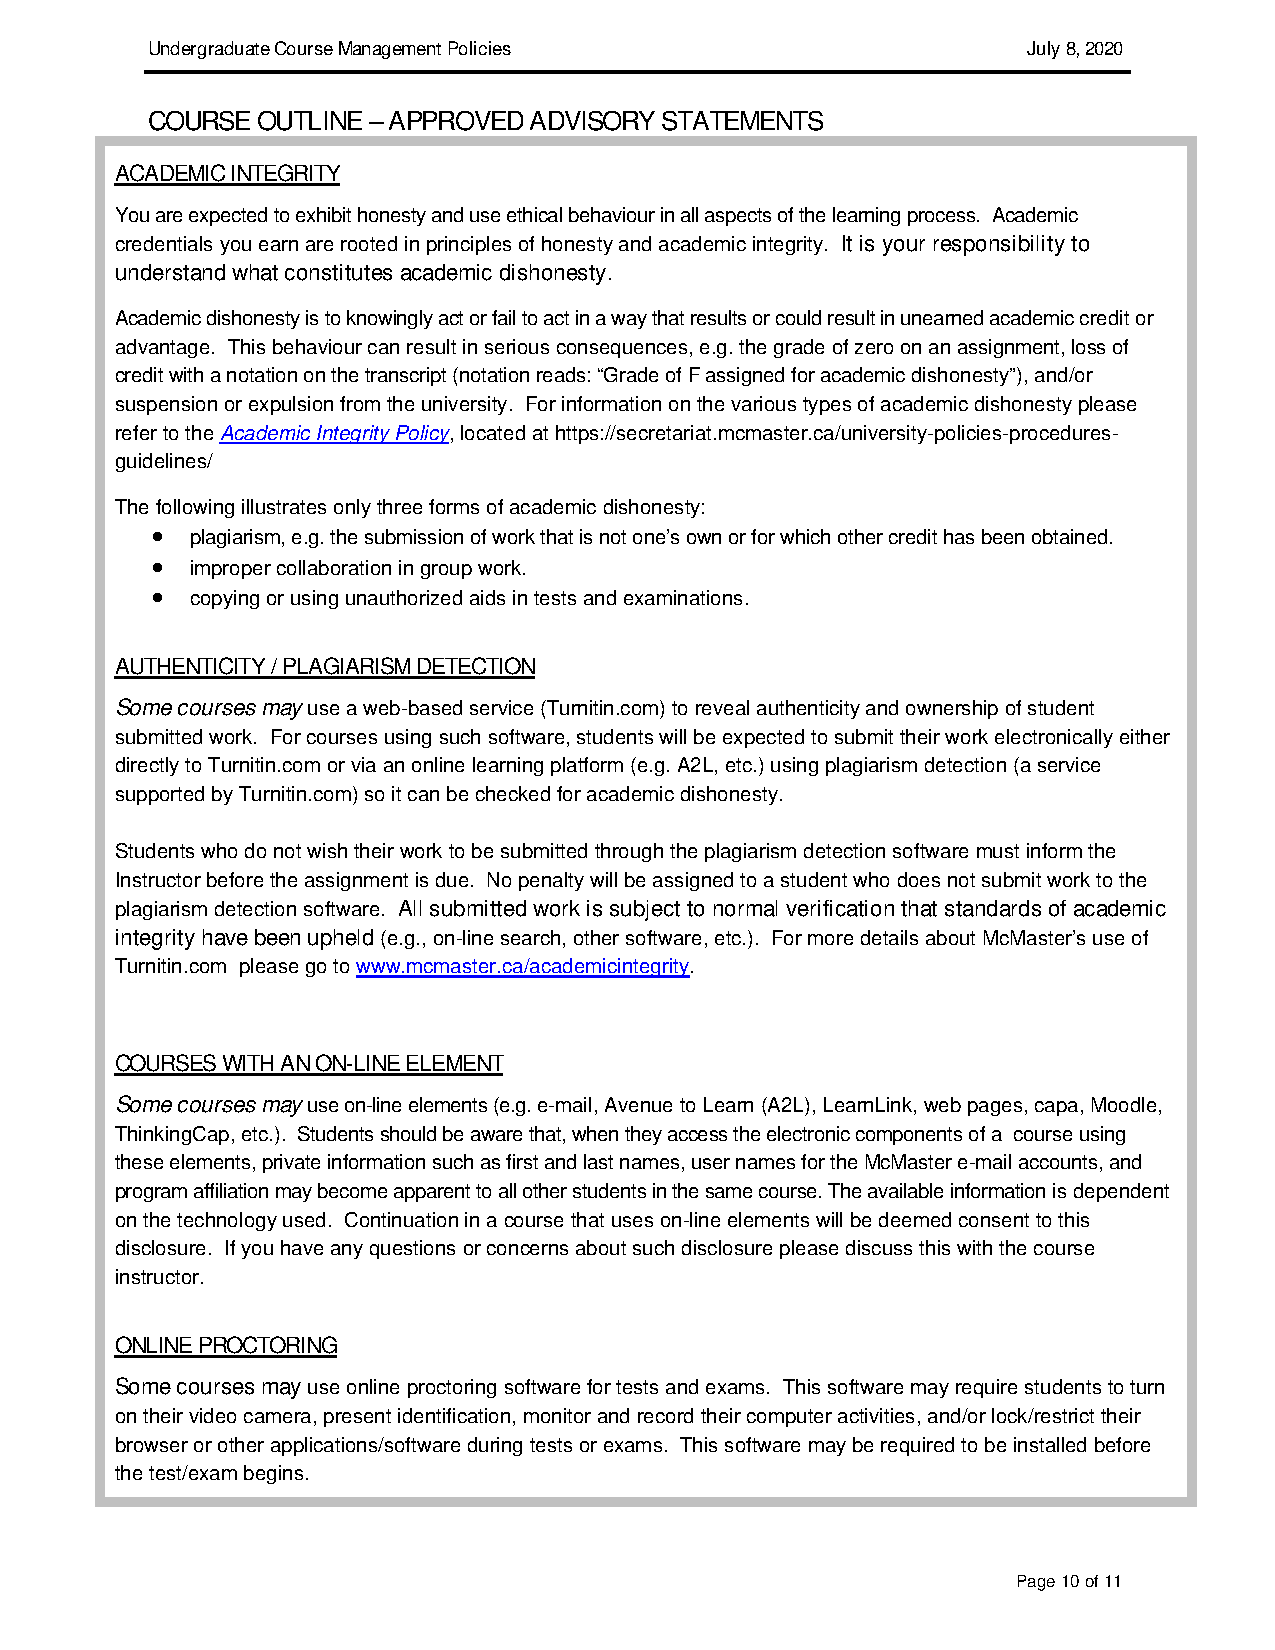
\includepdf[pages=-,width=\pagewidth]{media/outline-advisory-statements.pdf}
\end{document}
